\documentclass[12pt,a4paper]{article}

\usepackage{jyw-program}

\begin{document}
\title{猜數字遊戲:幾A幾B}
\author{Jia-Yin Wang}
\maketitle

\begin{abstract}
這份講義探討幾A幾B的猜數字遊戲,主要對象是初學程式設計的同學。為了方便理解,我們使用3個數字的例子來做說明,同學理解之後可以將其加以擴充。
\end{abstract}

\section{人猜,電腦回答}

電腦選定一個不重複的三位數(首位可以為0)當作答案,使用者每次猜答,電腦會根據答案給出幾A幾B的提示。A表示數字相同且位置正確的個數,B表示數字相同但位置錯誤的個數。例如:如果答案是123,但猜的是325,則回答1A1B。使用者必須根據提示一直猜,直到猜中為止。
\begin{figure}[H]
	\centering
	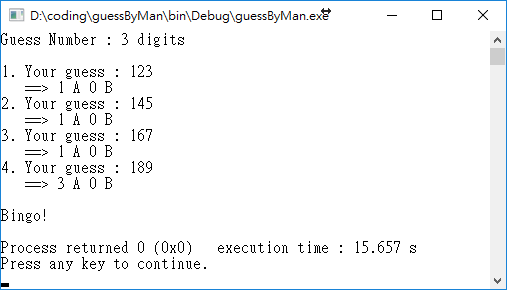
\includegraphics{Fig/man}
\end{figure}

\subsection{解題思惟}
因為是猜數字遊戲,所以希望每次設定的數字都不相同。那麼要如何產生不同的亂數呢?一般來說,我們會使用 rand() 函式來得到一個隨機的整數,那如果我們要取 0-9 的亂數的話,我們可以使用它除以 10 的餘數。

rand() 函式實際上會使用一個預設的整數當種子值,把它用來做一些計算之後會得到另一個整數,做為我們的亂數輸出,並且也把它設為新的種子值,用來計算下一個亂數。如果我們沒有特別設定亂數的種子值,因為預設值都一樣,這樣每次程式產生的亂數序列都會相同。

那要怎麼設定種子值呢?基本上我們是使用 srand(seed) 來設定,這邊 seed 是做為種子值的整數。如果我們設定不同的種子值,那產生的序列就會和之前的不一樣,不過因為種子值仍是固定的,所以每次執行的結果仍會相同。

那如何讓每次執行出來的亂數都不同呢?基本上我們常用的方法是使用 srand(time(NULL)) 來設種子值。這邊 time(NULL) 是一個時間函數,會返回
從1970年1月1日00:00:00一直到現在所經歷的秒數,拿這個來做為種子值,因為每次開始執行的時間不同,所產生出來的序列就不一樣了。

此處須注意:使用 rand() 及 srand() 函式要引入 <stdlib.h>,使用 time(NULL) 函式要引入 <time.h>。
\subsubsection{程式流程:}
\begin{enumerate}
	\item 取得一個不重複的三位數。
	\item 讓使用者輸入猜的數字。
	\item 計算幾個A。
	\item 計算幾個B。
	\item 若沒有猜中,則回到步驟2,繼續下一回合。
	\item 猜中的話,印出成功的訊息並結束程式。
\end{enumerate}

\subsubsection{函式說明:}
\vspace{0.5cm}
\begin{enumerate}
	\item int getRand3()
	
	怎樣取得一個不重複的 3 位數呢?我們可以一次取一位 0-9 的亂數,那如果取出來的數之前曾出現過,就重新再取,等取得3個不同的數字之後,將其組合,就是一個不重複的 3 位數。

	\item int countA(int guess, int ans)
	
	此函數用來計算幾個A。參數guess是使用者猜的數字,ans是答案。使用\%10分別取得guess及ans的個位數,比較兩數,若相等,則cnt++。比較完之後將guess及ans分別除以10,將其個位去掉,再重複同樣的運算。因為guess及ans是一個三位數,所以用for迴圈執行3次比較。最後輸出cnt即可知道猜中幾個A。
	
	\item int countB(int guess, int ans)
	
	此函數用來計算幾個B。將guess及ans的個位、十位及百位數分別存入陣列a及陣列b。使用雙重for迴圈掃描所有陣列a和陣列b的配對比較,若位置不同(i != j)且數字相同(a[i] == b[j]),則cnt++。最後輸出cnt即可知道猜中幾個B。
\end{enumerate}

\subsection{程式碼}
\begin{cppcode}
	#include <iostream>
	#include <cstdlib>
	#include <ctime>
	
	using namespace std;
	
	int getRand3();
	int countA(int guess, int ans);
	int countB(int guess, int ans);
	
	int main()
	{
		int mynumber, yourguess, idx=1;
		cout << "Guess Number : 3 digits\n\n";
		mynumber = getRand3();
		do {
			cout << idx++ << ". Your guess : ";
			cin >> yourguess;
			int a = countA(mynumber, yourguess);
			int b = countB(mynumber, yourguess);
			cout << "   ==> " << a << " A " << b << " B" << endl;
		} while (yourguess != mynumber);
		cout << endl << "Bingo!" << endl;
		return 0;
	}
	
	int countA(int guess, int ans)
	{
		int d1, d2, cnt=0;
		for (int i=0; i<3; i++) {
			d1 = guess % 10;
			d2 = ans % 10;
			if (d1==d2) cnt++;
			guess /= 10;
			ans /= 10;
		}
		return cnt;
	}
	
	int countB(int guess, int ans)
	{
		int a[3], b[3], cnt=0;
		for (int i=0; i<3; i++) {
			a[i] = guess % 10;
			b[i] = ans % 10;
			guess /= 10;
			ans /= 10;
		}
		for (int i=0; i<3; i++) {
			for (int j=0; j<3; j++) {
				if (i!=j && a[i]==b[j]) cnt++;
			}
		}
		return cnt;
	}
	
	int getRand3()
	{
		int a, b, c;
		srand(time(NULL));
		a = rand() % 10; // 0--9
		do {
			b = rand() % 10;
		} while (b==a);  // if b==a, re-choose b
		do {
			c = rand() % 10;
		} while (c==a || c==b);  // if c==a or c==b, re-choose c
		return a*100+b*10+c;
	}
\end{cppcode}

\vspace{1cm}
\section{電腦猜,人回答}

使用者選定一個不重複的三位數(首位可以為0)當作答案,電腦每次猜答,使用者要根據答案給出幾A幾B的提示。A表示位置正確的數的個數,B表示數字正確但位置錯誤的數的個數。電腦根據提示一直猜,直到猜中為止。
\begin{figure}[H]
	\centering
	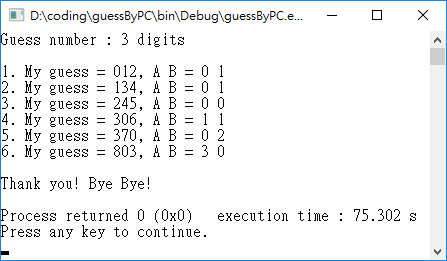
\includegraphics{Fig/PC}
\end{figure}

\subsection{解題思惟}
這次倒過來,讓電腦猜,有一點小小人工智慧的感覺。但是電腦怎麼猜呢?我們可以使用一個簡單的辦法,首先宣告一個1000個元素的陣列,其中位置0-999分別代表0-999所有的數。如果某個數不會是答案,我們就把那個數的位置設成0,如果有可能是答案,我們就把它設成1。那麼程式一開始時,可以先把有相同數字的三位數去掉,也就是把它的位置設成0,其他的都設成1。接著電腦從頭開始,找一個可能是答案的數字來猜,譬如說xyz,等使用者回答之後,我們再根據它的回答,把每個可能的數和xyz做比較,如果比出來的結果和使用者的回答有出入,那就不可能是答案,我們就把這些數去掉,然後電腦接著再找可能是答案的數字來猜。這樣一直重複下去,直到猜出來為止。
\subsubsection{程式流程:}
\begin{enumerate}
	\item 初始化陣列,將不可能成為答案的元素設成0,其他設成1。
	\item 輸出一個可能的答案。
	\item 讓使用者輸入幾A幾B。
	\item 若沒猜中,則根據幾A幾B將不可能的答案剔除,並回到步驟2。
	\item 若猜中的話,輸出提示訊息並結束程式。
\end{enumerate}

\subsubsection{函式說明:}
\begin{enumerate}
	\item void initCandidates()
	
	此函數用來初始化陣列。在0-999的整數中,分別取出個位、十位及百位數。若三個數字有重複,則不可能成為答案,將此元素設為0,其他元素設為1。
	
	\item int validGuess()
	
	此函數選出電腦猜的數字。用for迴圈掃描陣列,若是可能的答案,則回傳。
	
	\item updateCandidates(int number, int ga, int gb)
	
	此函數用來更新陣列。用for迴圈掃描陣列,若是可能的答案,判斷是否符合幾A幾B,若不符合,則將此元素設為0。
\end{enumerate}

\subsection{程式碼}
\begin{cppcode}
	#include <cstdio>
	
	int candidates[1000];
	
	void initCandidates();
	int  validGuess();
	void updateCandidates(int number, int ga, int gb);
	int  countA(int guess, int ans);
	int  countB(int guess, int ans);
	
	int main()
	{
		int guess, idx=1, a, b;
		
		initCandidates();
		printf("Guess number : 3 digits\n\n");
		do {
			guess = validGuess();
			printf("%d. My guess = %03d, A B = ", idx++, guess);
			scanf("%d%d", &a, &b);
			updateCandidates(guess, a, b);
		} while (a!=3 || b!=0);
		printf("\nThank you! Bye Bye!\n");
		
		return 0;
	}
	
	// init candidates, erase all number with same digit
	void initCandidates()
	{
		for (int n=0; n<1000; n++) {
			int a = n/100;       // a..
			int b = (n/10) % 10; // .b.
			int c = n % 10;      // ..c
			if (a==b || b==c || c==a) candidates[n]=0;
			else candidates[n]=1;
		}
	}
	
	int validGuess()
	{
		for (int i=0; i<1000; i++) {
			if (candidates[i]) return i;
		}
		return -1; // No possible candidate
	}
	
	void updateCandidates(int number, int ga, int gb)
	{
		for (int i=0; i<1000; i++) {
			if (candidates[i]) {
				if (ga != countA(number, i)) candidates[i] = 0;
				if (gb != countB(number, i)) candidates[i] = 0;
			}
		}
	}
	
	int countA(int guess, int ans)
	{
		int d1, d2, cnt=0;
		for (int i=0; i<3; i++) {
			d1 = guess % 10;
			d2 = ans % 10;
			if (d1==d2) cnt++;
			guess /= 10;
			ans /= 10;
		}
		return cnt;
	}
	
	int countB(int guess, int ans)
	{
		int a[3], b[3], cnt=0;
		for (int i=0; i<3; i++) {
			a[i] = guess % 10;
			b[i] = ans % 10;
			guess /= 10;
			ans /= 10;
		}
		for (int i=0; i<3; i++) {
			for (int j=0; j<3; j++) {
				if (i!=j && a[i]==b[j]) cnt++;
			}
		}
		return cnt;
	}
	
\end{cppcode}

\end{document}
